\documentclass[twocolumn]{jsarticle}
\usepackage{graphicx}
%\usepackage[superscript]{cite}  %参考文献番号を上付にしないなら要らない
% \renewcommand\citeform[1]{[#1]} %cite.styを使わないときにはこれもコメントにすること
%\usepackage{times} % TimesとHelveticaを使う.数式はComputer Modern
%\usepackage{bm} % \bm{}で数式モードでboldを使う.
\usepackage{aic2022}
%\usepackage{here} %here.styがあると図を指定位置に入れられる.[!htbp]の代わりに[H]

\title{発表のタイトル}
\author{西川$^1$,日吉花子$^1$,三田二郎$^2$}
\affiriation{$^1$慶應義塾大学〇〇学部〇〇学科\\$^2$慶應義塾大学大学院〇〇研究科〇〇専攻}
\abst{概要を4行前後で記述する\\
このテンプレートに厳密に準拠する必要はありません.
余白の大きさや段組み,字体や大きさ,図表番号や参考文献の表記法の
目安として参照してください.研究発表の論文は6ページ,ポスター発表
の要旨は1ページを目安に仕上げて頂きたいですが,ページ数に過不足
があっても構いません.なお,ヘッダやフッタ領域には
カンファレンス実行委員側で会議名やページ数などを付け加えますので,
著者はページ数などを記載しないでください.
}
\keywords{英語のキーワードを3から5単語記述する}
\begin{document}
\maketitle

\section{研究背景・目的}
「何をやるのか」「どうしてやるのか」研究の目的・意義を明確かつ論理的に述べる.
そのためには,研究背景を述べ,先行研究\cite{bunken1}でどこまで明らかにされているか説明することが必要である.
研究の意義を説く説得力のある序論を書くことが,良い要旨を書くための鍵となる\cite{bunken2}.

論文の構成は砂時計形なので,最初は誰もが納得する一般的な事実のように大きな話題から始めて,次第に絞り込んでこの研究の目的に持っていく.
そのときに,論理の飛躍がないように注意する.

\section{方法}
研究方法の概要を説明する(過去形).
第3者が再現するに足りる情報を記載する.
必要に応じて小節に分ける.

(ここから意味のない文)

あいうえお かきくけこ さしすせと たちつてと なにぬねの まみむめも やゆよ らりるれろ わをん

あいうえお かきくけこ さしすせと たちつてと なにぬねの まみむめも やゆよ らりるれろ わをん

あいうえお かきくけこ さしすせと たちつてと なにぬねの まみむめも やゆよ らりるれろ わをん

あいうえお かきくけこ さしすせと たちつてと なにぬねの まみむめも やゆよ らりるれろ わをん

あいうえお かきくけこ さしすせと たちつてと なにぬねの まみむめも やゆよ らりるれろ わをん

あいうえお かきくけこ さしすせと たちつてと なにぬねの まみむめも やゆよ らりるれろ わをん

あいうえお かきくけこ さしすせと たちつてと なにぬねの まみむめも やゆよ らりるれろ わをん
(ここまで意味のない文)

\section{結果}
\subsection{結果1}
Figure \ref{fig:voltage}のように得られた結果を提示する.
紙面が限られているため,結論を伝えるのに最も重要な結果のみを示す.
図表を適切に用い,結果を分かりやすく伝える.
図表に示しただけで,著者の主張したいことの説明がないのは不適切である.
主張したいことに沿って,図表から読み取れる客観的な事実を説明する.

\begin{figure}[!htbp]
\centering
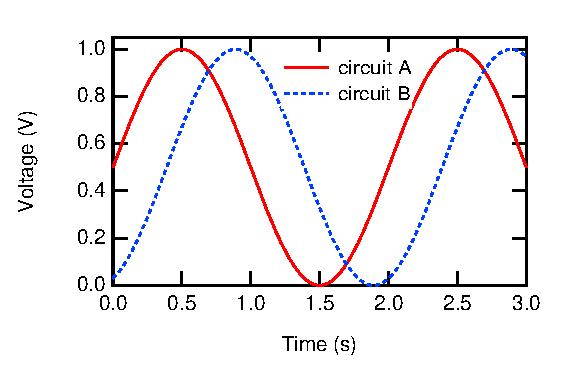
\includegraphics[width=0.9\columnwidth]{voltage.eps}
\caption{Time dependence of output voltage}
\label{fig:voltage}
\end{figure}

図の文字は小さくなりすぎないようにする.

\subsection{結果2}
必要に応じて,章をさらに細かい節に分ける(Table \ref{tbl:radii}参照).
\begin{table}[!htbp]
\centering
\caption{Radii of fabricated samples}
\label{tbl:radii}
\begin{tabular}{c|c}
\hline
& Radius (mm) \\
\hline
Sample A & 45 \\
Sample B & 38 \\
\hline
\end{tabular}
\end{table}

\section{考察}
方法や結果の妥当性を議論する.
他の文献と比較など,客観的な事実を用いる.
合理的な推論は許容範囲であるが,客観的な事実で書けるならその方が良い.

方法や結果に記していない自身の新しい実験方法や結果を考察でいきなり書かない.
比較する必要や検証に用いる必要があるなら方法や結果に書く.

研究背景・目的でも述べたように,論文の構造は砂時計形なので,最初にこの論文に関することについて記載し,最後に向かってより大きな一般的な話題に進める.


\section{結論(と今後の展望)}
最も主要な結論を簡潔に述べる.研究目的に対して,どのような結論が得られたか明確に記述することが重要である.必要に応じて,今後の展望を述べる.

\begin{thebibliography}{9}
\bibitem{bunken1} S. Yagami, Science, \textbf{393}, 113--117 (1998).
\bibitem{bunken2} S. Yagami \textit{et al}., Proc. IEEE \textbf{52}, 284--290 (2013).
\end{thebibliography}
\end{document}

